\section{Tasks}


\subsection{}
Разработать подпрограмму генерации регулярных и адаптивных сеточных разбиений произвольного отрезка \([a, b]\) в зависимости от числа сегментов разбиения и величины коэффициента разрядки \(r\)
\begin{figure}
	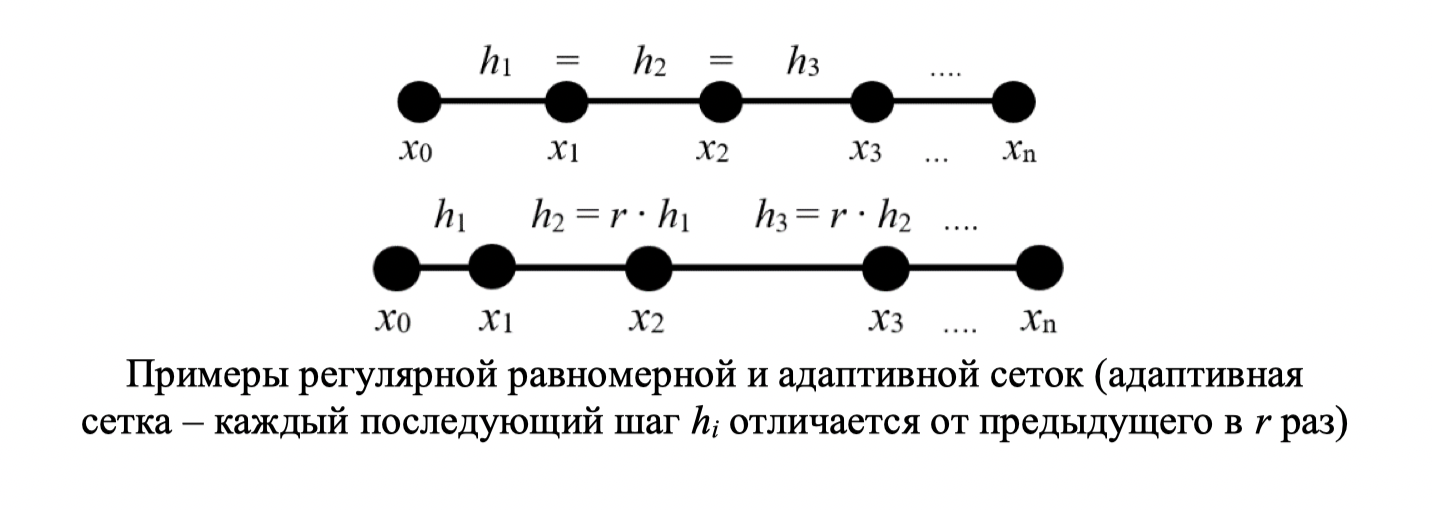
\includegraphics[width=\linewidth, height=7cm]{images/imaget1.png}
	\caption{Взято из учебного пособия}
\end{figure}

\subsection{}
Кусочно-полиномиальная интерполяция. Разработать класс, реализующий интерфейс кубического интерполяционного сплайна с непрерывными первой и второй производными и удовлетворяющего краевым условиям нулевой кривизны \(S'' (a) = S'' (b) = 0\).

\subsection{}
Для набора аналитических функций \(f(x) = x, x^2, x^3, x^4, sin(x)\) провести исследования на вложенных сетках. Для этого задайте шаг h и постройте равномерное сеточное разбиение отрезка \([a, b]\). Получите таблицу значений сплайна и его двух первых производных в точках, которые НЕ совпадают с узловыми (не менее 10). Повторить данные исследования на сетках с шагом \(h/2\) и \(h/4\). Полученные результаты сопоставьте с аналитической оценкой точности сплайн-аппроксимации: если \(f(x)\in C^{k + 1}[a, b]\), \(0 \leq k \leq 3\), то для интерполяционного сплайна \(S(x)\) выполнено \(max _{x\in [a,b] }|f(^{(m)}(x) − S^{(m)}(x)| \leq Ch^{k+1-m} max_{x\in [a,b] }|f^{(m)}(x)|, C - const\) т.е. погрешность аппроксимации ограничена сверху величиной \(O(h^{k+1-m})\) при ограниченной \(m\)-ой производной аппроксимируемой функции. В отчёте привести величину шага \(h\) и соответствующую норму погрешности аппроксимации.

\subsection{}
Выяснить как влияет на вторую производную сгущение сетки к концам отрезка \([a,b]\).

\subsection{}
Сглаживание и аппроксимация МНК. Разработать класс, реализующий интерфейс сглаживающего сплайна. На каждом сегменте разбиения использовать базисную систему финитных функций первого порядка. Сглаживающий сплайн \(g(x)\) строить как решение задачи о минимизации функционала в линейном подпространстве \(\Omega \subset C[a,b] \hspace{1em} \Phi=(1−p)||f(x)−g(x)||^2_2+p||g'(x)||^2_2\)
, где \(p\) – параметр сглаживания.

\subsection{}
Для сильно осциллирующей функции \(f(x)=x|sin(10000x)|\), \(x\) – радианы, на одной диаграмме изобразить интерполяционный и сглаживающий сплайны. Параметр сглаживания \(p\) варьировать от 0 до 1. Использовать равномерную сетку с шагом \(h\) и \(h/2\).

\subsection{}
Выяснить, на что влияет варьирование весовых коэффициентов в дискретном скалярном произведении при построении сглаживающего сплайна.
